\chapter{Results and Discussion}

We have reviewed the rich history of hadronic (QCD?) spin physics and identified
the need to more precisely constrain the polarized gluon distribution. We
described the experimental apparatus and the analysis techniques used to collect
and study millions of polarized proton collisions towards that end. This chapter
presents the final results of the analysis, a set of asymmetries that are
directly sensitive to polarized glue and allow a deeper understanding of the
fundamental nature of QCD in the nucleon.

\section{$A_{LL}$ for Inclusive Charged Pion Production}

Figure~\ref{fig:final-result-run5} presents the first measurement of \(A_{LL}\)
for inclusive charged pion production at the STAR experiment. The data are
plotted versus the \(p_T\) of the pion and are compared to a variety of NLO pQCD
predictions \cite{}. The dashed black curve represents a prediction for
\(A_{LL}\) based on the GRSV Standard parameterization of \(\Delta g(x)\), which
was derived in 2001 from a global fit to polarized DIS data. The MIN and ZERO
curves correspond respectively to maximally negative and zero gluon polarization
in the nucleon. Not shown is the fourth member of the GRSV set, corresponding to
maximal gluon polarization, which has been excluded by earlier measurements of
\(A_{LL}\) in other final-state channels (and is similarly excluded by this
measurement).

The dashed magenta curve labeled GS Set C is based on a polarized gluon
distribution by Gehrmann and Stirling that has a small integral polarization in
the \(x\) range accessible to 200 GeV mid-rapidity measurements at RHIC, but in
fact has a very large polarization content at smaller values of \(x\). Future
correlation measurements and measurements at a 500 GeV center-of-mass energy
will enable STAR to test whether distribution functions of this form might
correspond to reality. Finally, the solid black curve represents a new
parameterization of \(\Delta g(x)\) by de Florian, Sassot, Stratmann, and
Vogelsang which is based on a global fit incorporating both DIS data and early
\(A_{LL}\) results from RHIC.\footnote{The measurements in this thesis are not
included in the current DSSV global fit.}

\begin{figure}[ht]
  \includegraphics[width=1.0\textwidth]{figures/final-result-run5}
  \caption{$A_{LL}$ for inclusive charged pion production as a function of pion $p_T$.  The error bars represent statistical uncertainties while the gray bands display total point-to-point systematic uncertainties.  The data are compared to NLO pQCD predictions incorporating various models for $\Delta g(x)$ \cite{}.}
  \label{fig:final-result-run5}
\end{figure}

\section{$A_{LL}$ for Jet + Pion Correlations}

Shown in Figure~\ref{fig:final-result-run6} are STAR's first measurements of
\(A_{LL}\) for charged pions opposite a trigger jet. The data are plotted versus
the fragmentation variable \(z\), using the away-side trigger jet \(p_T\) as a
surrogate for the \(p_T\) of the parton from which the pion fragmented. NLO pQCD
predictions for the measurement are plotted assuming the GRSV Standard, GS Set
C, and DSSV gluon distributions discussed above. The large difference in the
predictions for \(\pi^-\) \(A_{LL}\) and \(\pi^+\) \(A_{LL}\) at high \(z\) is a
reflection of the importance of favored fragmentation in that regime. Recall
that the \(\Delta u(x)\) distribution in the proton is uniformly positive, while
the \(\Delta d(x)\) distribution is smaller and uniformly negative. At high
\(z\), where the disparity between favored and disfavored fragmentation is
large, the \(\pi^-\) \(A_{LL}\) is driven by \(d\) quark scattering and the
\(\pi^+\) by \(u\) quark scattering. Favored fragmentation is also responsible
for the very different functional forms of the MIN \(A_{LL}\) prediction for
inclusive \(\pi^-\) and \(\pi^+\) \(A_{LL}\) in
Figure~\ref{fig:final-result-run5}.

\begin{figure}[]
  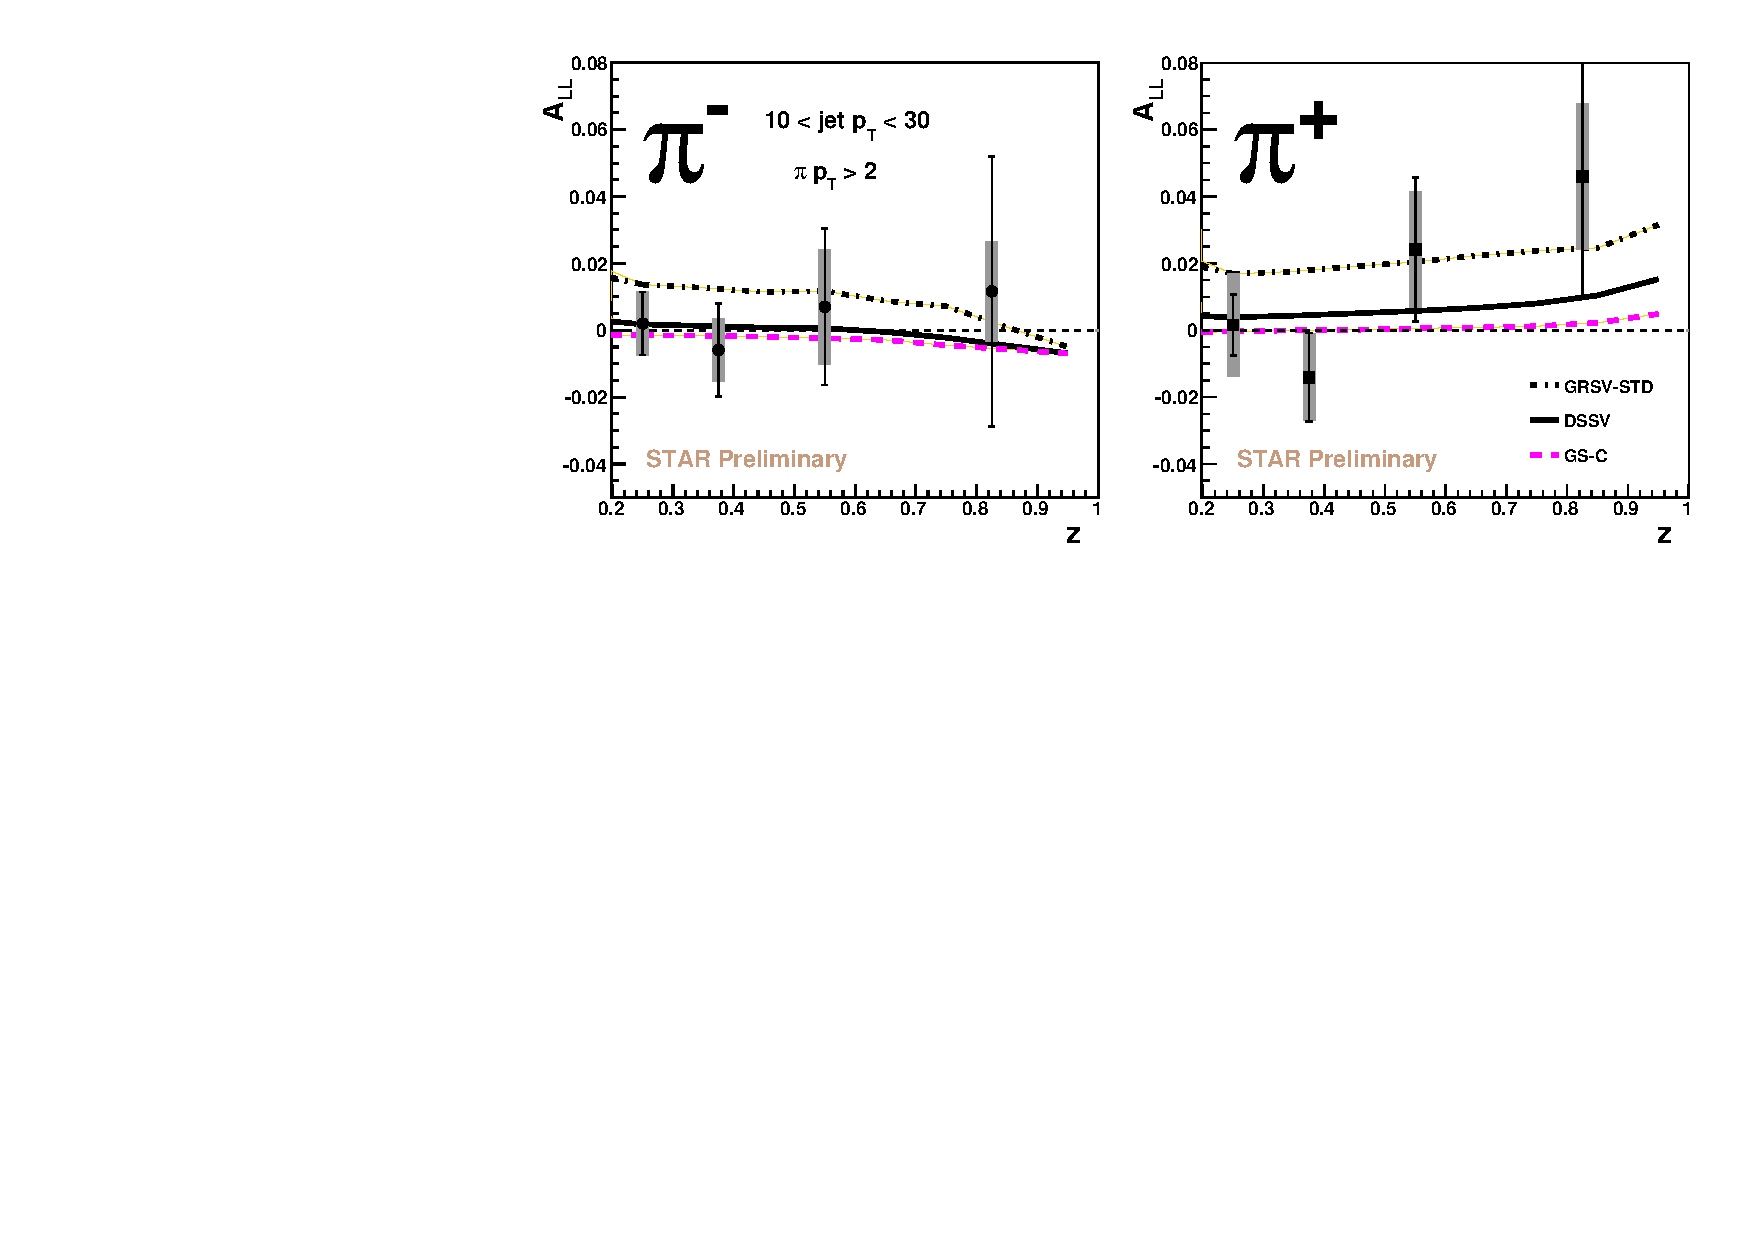
\includegraphics[width=1.0\textwidth]{figures/final-result-run6-3}
  \caption{$A_{LL}$ for charged pion production opposite an identified jet.  The data are plotted against the ratio of the pion and jet transverse momenta, here labeled using the fragmentation variable $z$.  As in Figure~\ref{fig:final-result-run5}, the error bars represent statistical uncertainties and the gray bands point-to-point systematics.  The NLO predictions are the result of a recent analysis by de Florian \cite{}.}
  \label{fig:final-result-run6}
\end{figure}

\begin{table}
  \centering
  \begin{tabular}{|c||c|c|c||c|c|c|}
    \hline
    \multirow{2}{*}{$p_T$} & \multicolumn{3}{c||}{$\pi^{-}$} & \multicolumn{3}{c|}{$\pi^{+}$} \\
    \cline{2-7}
    & $A_{LL}$ & Stat. Error & Syst. Error &$A_{LL}$ & Stat. Error & Syst. Error\\
    (GeV/c) & ($10^{-3}$) & ($10^{-3}$) & ($10^{-3}$) & ($10^{-3}$) & ($10^{-3}$) & ($10^{-3}$) \\
    \hline
    \hline
    2.00 - 3.18 & -5.5 & $\pm$ 6.3 & -6.7 +4.1 
                &  -3.3 & $\pm$ 6.1 & -6.3 +6.3\\
    3.18 - 4.56 & 1.6 & $\pm$ 9.9 & -8.7 +7.6 
                &  -1.5 & $\pm$ 9.5 & -13.1 +7.1\\
    4.56 - 6.32 & 0.0 & $\pm$ 15.9 & -10.1 +5.1 
                &  3.1 & $\pm$ 15.2 & -18.6 +11.8\\
    6.32 - 8.80 & -48.9 & $\pm$ 26.4 & -9.4 +7.0 
                &  -1.9 & $\pm$ 25.2 & -21.7 +19.5\\
    8.80 - 12.84 & -33.0 & $\pm$ 49.4 & -13.0 +13.4 
                &  -72.8 & $\pm$ 48.5 & -21.5 +16.4\\
    \hline
  \end{tabular}
  \caption{$A_{LL}$ for inclusive charged pion production.}
  \label{tab:final-2005-result}
\end{table}

\begin{table}
  \centering
  \begin{tabular}{|c||c|c|c||c|c|c|}
    \hline
    \multirow{3}{*}{$z$} & \multicolumn{3}{c||}{$\pi^{-}$} & \multicolumn{3}{c|}{$\pi^{+}$} \\
    \cline{2-7}
    & $A_{LL}$ & Stat. Error & Syst. Error &$A_{LL}$ & Stat. Error & Syst. Error\\
    & ($10^{-3}$) & ($10^{-3}$) & ($10^{-3}$) & ($10^{-3}$) & ($10^{-3}$) & ($10^{-3}$) \\
    \hline
    \hline
    0.20-0.30 &  2.0 & $\pm$ 9.4 & $\pm$ 9.6 
              &  1.6 & $\pm$ 9.1 & $\pm$ 15.3 \\
    0.30-0.45 & -5.9 & $\pm$ 13.9 & $\pm$ 9.5 
              & -14.1 & $\pm$ 13.2 & $\pm$ 13.1 \\
    0.45-0.65 &  7.0 & $\pm$ 23.4 & $\pm$ 17.1 
              &  24.1 & $\pm$ 21.5 & $\pm$ 17.3 \\
    0.65-1.00 &  11.6 & $\pm$ 40.4 & $\pm$ 14.9 
              &  46.0 & $\pm$ 36.5 & $\pm$ 21.8 \\
    \hline
  \end{tabular}
  \caption{$A_{LL}$ for charged pions opposite a trigger jet.}
  \label{tab:final-2006-result}
\end{table}

\section{Interpretation and Future Work}

